% 原书印刷63--67页，PDF物理90--94页，止于2.3标题之前.
\subsection{单调映射的最优性}\label{sec:2.2}\index{M103@单调映射（monotone map）|hyperpage}

现在我们已相当清楚地了解映射$\mathrm T_{\rm mon}$与方案$\gamma_{\rm mon}$的性质、定义及刻画，可以看到，在一维中，它们对于多种不同成本都是最优的，而不仅仅对二次成本如此. 这确实是一维情形特有的现象，在高维并不成立. 我们考虑的成本是差$x-y$的凸函数；为强调这些成本可能具有非对称性，宁愿将其写成$h(y-x)$，而不是$h(x-y)$.

\begin{theorem}\label{obj:2.9}\index{C029@凸传输成本（convex transport costs）|hyperpage}\index{E058@最优映射的存在性（existence of an optimal map）|hyperpage}
设$h:\mathbb R\to\mathbb R_+$严格凸，$\mu,\nu\in\mathscr P(\mathbb R)$为概率测度. 考虑成本$c(x,y)=h(y-x)$，并假设(KP)的值有限. 则(KP)有唯一解，且该解为$\gamma_{\rm mon}$. 若$\mu$无原子，这个最优方案由映射$\mathrm T_{\rm mon}$诱导.

此外，若去掉严格凸性假设，只要求$h$凸，则同一个$\gamma_{\rm mon}$仍然是最优运输方案，但不再保证唯一性.
\end{theorem}
\begin{proof}
利用任意最优$\gamma$的支集都是$c$-循环单调集$\Gamma$这一事实. 这特别意味着，对$(x,y),(x',y')\in\Gamma$，有
\begin{equation}\label{eq:2.3}\index{0007@$c$-循环单调性（$c$-cyclical monotonicity）|hyperpage}
h(y-x)+h(y'-x')\le h(y'-x)+h(y-x').
\end{equation}
只需证明，在严格凸情形下，这蕴含单调性：实际上，将由\eqref{eq:2.3}推出$x<x'$蕴含$y\le y'$，从而借助\autoref{obj:2.8}得出结论.

为证明$y\le y'$，反设$y>y'$，记$a=y-x$、$b=y'-x'$及$\delta=x'-x>0$. 条件\eqref{eq:2.3}变为$h(a)+h(b)\le h(b+\delta)+h(a-\delta)$. 此外，$y'<y$意味着$b+\delta<a$. 因而$b+\delta$和$a-\delta$都位于$b$与$a$之间的线段上（且$b<a$）. 更准确地，
\[
b+\delta=(1-t)b+ta,\qquad a-\delta=tb+(1-t)a,
\qquad t=\frac{\delta}{a-b}\in]0,1[.
\]
于是严格凸性给出
\[
\begin{aligned}
h(a)+h(b)&\le h(b+\delta)+h(a-\delta)\\
&<(1-t)h(b)+th(a)+th(b)+(1-t)h(a)\\
&=h(a)+h(b).
\end{aligned}
\]
这产生矛盾，从而证明严格凸情形的陈述.

若$h$仅凸，则当$h$为常数时，结论显然成立（因为每个$\gamma$都最优）；否则可通过逼近得到结论. 下面的\autoref{obj:2.10}表明，存在一列严格凸函数$h_\varepsilon$满足$h\le h_\varepsilon\le(1+\varepsilon)h+\varepsilon$. 取运输成本$c_\varepsilon(x,y):=h_\varepsilon(y-x)$. 已知$\gamma_{\rm mon}$使成本$\int c_\varepsilon\,d\gamma$最优，因此对所有$\gamma\in\Pi(\mu,\nu)$，有
\[
\begin{aligned}
\int h(y-x)\,d\gamma_{\rm mon}
&\le\int h_\varepsilon(y-x)\,d\gamma_{\rm mon}
\le\int h_\varepsilon(y-x)\,d\gamma\\
&\le\varepsilon+(1+\varepsilon)\int h_\varepsilon(y-x)\,d\gamma.
\end{aligned}
\]
令$\varepsilon\to0$，得到$\gamma_{\rm mon}$也使成本$c$最优.
\end{proof}

\begin{lemma}\label{obj:2.10}
对每个非常值的正凸函数$h:\mathbb R\to\mathbb R_+$及每个$\varepsilon>0$，存在严格凸的$h_\varepsilon:\mathbb R\to\mathbb R_+$，使$h\le h_\varepsilon\le(1+\varepsilon)h+\varepsilon$.
\end{lemma}
\begin{proof}
只需证明存在严格凸函数$f:\mathbb R\to\mathbb R_+$满足$f\le h+1$. 然后取$h_\varepsilon:=h+\varepsilon f$. 由于$h$凸，它有仿射下界，且有$h(t)\ge(at+b)_+$（因已知$h\ge0$，故可取正部）. 可以验证，
\[
f(t):=\frac12\sqrt{4+(at+b)^2}+\frac12(at+b)
\]
严格凸，且满足$f(t)\le\frac12(2+|at+b|+(at+b))=1+(at+b)_+$.
\end{proof}

\begin{remark}\label{obj:2.11}
只要$\mu$与$\nu$满足某些可积性条件，使$\inf\textup{(KP)}> -\infty$，函数$h$的正性实际上并非必要. 例如，若$\int|x|\,d\mu(x),\int|y|\,d\nu(y)<+\infty$，就可以给$h$加上一个仿射函数而使它凸；这一仿射函数的成本有限且不依赖于$\gamma$（见下面的\autoref{obj:2.14}）.
\end{remark}

\begin{remark}\label{obj:2.12}
强调一下，完全类似的证明可以用来说明：严格凹成本（形如$h(y-x)$且$h$严格凹）的最优映射是单调递减，而不是单调递增的. 可与\autoref{sec:3.3.2}的描述比较.
\end{remark}

\begin{remark}\label{obj:2.13}\index{T153@扭曲条件（twist condition）|hyperpage}
$\gamma_{\rm mon}$的最优性也在更一般的假设下成立，即某些不具有$h(x-y)$形式、但满足扭曲条件的成本也如此. 见\autoref{ex:10}.
\end{remark}

下面可以构造一些简单例子，其中$c$凸但不严格凸，且$\mathrm T_{\rm mon}$不是唯一的最优运输映射.

\begin{example}[线性成本]\label{obj:2.14}
假设$c(x,y)=L(x-y)$，其中映射$a:\mathbb R^d\to\mathbb R$为线性映射. 此时每个运输方案$\gamma$都最优，每个运输映射也都最优. 只需写出
\[
\int L(x-y)\,d\gamma
=\int L(x)\,d\gamma-\int L(y)\,d\gamma
=\int L(x)\,d\mu-\int L(y)\,d\nu,
\]
即可看出结果不依赖于$\gamma$，只依赖于它的边缘测度. 这一一般例子对紧支撑的$\mu,\nu$（这样不会遇到$L(x)$与$L(y)$的可积性问题）以及任意维数都适用，因而也适用于一维.
\end{example}

\begin{example}[直线上的距离成本]\label{obj:2.15}
假设$c(x,y)=|x-y|$，且$\mu,\nu\in\mathscr P(\mathbb R)$满足$\sup\operatorname{spt}(\mu)<\inf\operatorname{spt}(\nu)$. 此时每个运输方案$\gamma$都最优，每个运输映射也最优. 只需注意，对每个$(x,y)\in\operatorname{spt}(\mu)\times\operatorname{spt}(\nu)$，有$c(x,y)=y-x$；这又是线性成本.
\end{example}

\begin{example}[移动书籍]\label{obj:2.16}
考虑$c(x,y)=|x-y|$、$\mu=\frac12\mathscr L^1_{[0,2]}$及$\nu=\frac12\mathscr L^1_{[1,3]}$. 则$\mathrm T_{\rm mon}(x)=x+1$是把$\mu$运输到$\nu$的单调运输方案. 其成本为$M(\mathrm T)=\int|\mathrm T_{\rm mon}(x)-x|\,d\mu=1$. 但由
\[
\mathrm T(x)=\begin{cases}x+2&\text{若 }x\le1,\\x&\text{若 }x>1\end{cases}
\]
给出的运输映射$\mathrm T$也满足$\mathrm T_\#\mu=\nu$，且$\int|\mathrm T(x)-x|\,d\mu=\frac12\int_0^1 2\,dx=1$，因而同样最优（\autoref{fig:2.1}）.
\end{example}

\begin{figure}[htbp]
\centering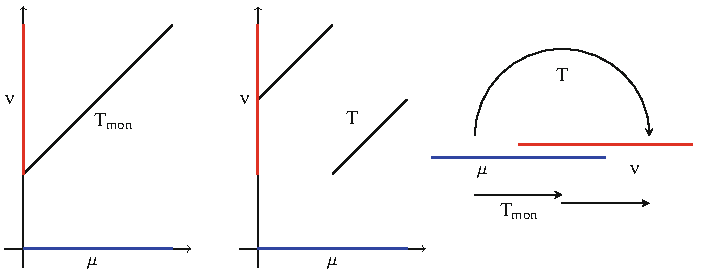
\includegraphics[width=\linewidth]{assets/ch02-fig-2-1.pdf}
\caption{移动书籍例子中的运输映射.}\label{fig:2.1}
\end{figure}

由上述各种成本的最优运输都是单调运输这一事实，可以用累积分布函数$F_\mu$与$F_\nu$，表示将给定测度$\mu$送到另一测度$\nu$的成本.

\begin{proposition}\label{obj:2.17}
给定$\mu,\nu\in\mathscr P(\mathbb R)$，考虑成本$c(x,y)=h(x-y)$，其中$h$为凸函数. 则有
\[
\mathscr T_c(\mu,\nu)=\int_0^1 h(F_\nu^{[-1]}-F_\mu^{[-1]})\,d\mathscr L^1.
\]
若$h(z)=|z|$，它还等于$\int_{\mathbb R}|F_\mu(t)-F_\nu(t)|\,dt$.
\end{proposition}
\begin{proof}
陈述的第一部分直接来自$\gamma_{\rm mon}$的最优性（\autoref{obj:2.9}）.

$h(z)=|z|$这一特殊情形可通过几何考虑处理：事实上，积分$\int_0^1|(F_\nu)^{-1}-(F_\mu)^{-1}|$等于带状区域$[0,1]\times\mathbb R$中由$(F_\mu)^{-1}$与$(F_\nu)^{-1}$的图像围成部分的面积. 为从反函数转到原函数，只需转过头来，沿变量$t$而不是$x$观察同一带状区域. 若想通过计算证明，则有
\[
\begin{aligned}
&\int|F_\nu^{[-1]}(x)-F_\mu^{[-1]}(x)|\,dx\\
&=\mathscr L^2\bigl(\{(x,t)\in[0,1]\times\mathbb R:
 F_\mu^{[-1]}(x)\le t<F_\nu^{[-1]}(x)\ \text{或}\ F_\nu^{[-1]}(x)\le t<F_\mu^{[-1]}(x)\}\bigr)\\
&=\mathscr L^2\bigl(\{(x,t)\in[0,1]\times\mathbb R:F_\mu^{[-1]}(x)\le t<F_\nu^{[-1]}(x)\}\bigr)\\
&\quad+\mathscr L^2\bigl(\{(x,t)\in[0,1]\times\mathbb R:F_\nu^{[-1]}(x)\le t<F_\mu^{[-1]}(x)\}\bigr).
\end{aligned}
\]
然后由Fubini定理，
\[
\begin{aligned}
&\mathscr L^2\bigl(\{(x,t)\in[0,1]\times\mathbb R:F_\mu^{[-1]}(x)\le t<F_\nu^{[-1]}(x)\}\bigr)\\
&=\int_{\mathbb R}\mathscr L^1\bigl(\{x\in[0,1]:x\le F_\mu(t)\ \text{且}\ F_\nu(t)<x\}\bigr)\,dt\\
&=\int_{\mathbb R}\mathscr L^1\bigl(\{x\in[0,1]:F_\nu(t)<x\le F_\mu(t)\}\bigr)\,dt.
\end{aligned}
\]
同样，
\[
\begin{aligned}
&\mathscr L^2\bigl(\{(x,t)\in[0,1]\times\mathbb R:F_\nu^{[-1]}(x)\le t<F_\mu^{[-1]}(x)\}\bigr)\\
&=\int_{\mathbb R}\mathscr L^1\bigl(\{x\in[0,1]:F_\mu(t)<x\le F_\nu(t)\}\bigr)\,dt.
\end{aligned}
\]
相加得到
\[
\begin{aligned}
&\mathscr L^2\bigl(\{(x,t)\in[0,1]\times\mathbb R:
 F_\mu^{[-1]}(x)\le t<F_\nu^{[-1]}(x)\ \text{或}\ F_\nu^{[-1]}(x)\le t<F_\mu^{[-1]}(x)\}\bigr)\\
&=\int_{\mathbb R}\mathscr L^1\bigl(\{x\in[0,1]:
F_\nu(t)<x\le F_\mu(t)\ \text{或}\ F_\mu(t)<x\le F_\nu(t)\}\bigr)\,dt\\
&=\int_{\mathbb R}|F_\mu(t)-F_\nu(t)|\,dt.
\end{aligned}
\]
证明完毕（\autoref{fig:2.2}）.
\end{proof}

\begin{figure}[htbp]
\centering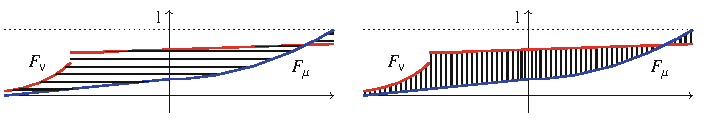
\includegraphics[width=\linewidth]{assets/ch02-fig-2-2.pdf}
\caption{\autoref{obj:2.17}最后一部分中的面积计算：$|F_\nu^{[-1]}-F_\mu^{[-1]}|$的积分对应于“水平地”看左图；若“竖直地”看，则得到$|F_\mu-F_\nu|$的积分.}\label{fig:2.2}
\end{figure}
